\documentclass[lmodern, utf8, zavrsni, numeric]{fer}
\usepackage{booktabs}
\usepackage{tikz}
\usetikzlibrary{matrix,chains,positioning,decorations.pathreplacing,arrows}
\usetikzlibrary{arrows.meta}
\usepackage{physics}


\usetikzlibrary{quotes,arrows.meta}


%%%NEWWW
\usepackage{amsmath}


\def\angle{30}
\def\scale{0.33}

\pgfmathsetmacro\sinangle{sin(\angle)}
\pgfmathsetmacro\cosangle{cos(\angle)}


\newcommand{\rect}[4]{
\def\l{#3}
\pgfmathsetmacro\ax{#1}
\pgfmathsetmacro\ay{#2}
\pgfmathsetmacro\bx{\ax}
\pgfmathsetmacro\by{\ay+\l}
\pgfmathsetmacro\cx{\bx+\cosangle*\l}
\pgfmathsetmacro\cy{\by+\sinangle*\l}
\pgfmathsetmacro\dx{\cx}
\pgfmathsetmacro\dy{\ay+\sinangle*\l}

\coordinate (a) at (\ax,\ay);
\coordinate (b) at (\bx,\by);
\coordinate (c) at (\cx,\cy);
\coordinate (d) at (\dx,\dy);

\begin{scope}[thick]
    \fill[draw=gray,fill=#4,opacity=0.5] (a) -- (b) -- (c) -- (d) -- cycle;
\end{scope}
}



\newcommand{\dmatrix}[6]{
	\pgfmathsetmacro\tox{#1+#4-1}
	\pgfmathsetmacro\toy{#2+#5-1}
    \foreach \i in {#1,...,\tox} {
	    \foreach \j in {#2,...,\toy} {
			\rect{\cosangle*#3+\i*\cosangle*\scale-\scale}{\i*\sinangle*\scale+\j*\scale-\scale}{\scale}{#6}
		}
    }
}

%NEWWWWWW

\usetikzlibrary{matrix,fit,calc}

\newcommand{\hhllineup}[4]{\draw (#1-#2-#3.north west) -- (#1-#2-#4.north east);}

\newcommand{\hhllinedown}[4]{\draw (#1-#2-#3.south west) -- (#1-#2-#4.south east);}

\newcommand{\vvllineleft}[4]{\draw (#1-#3-#2.north west) -- (#1-#4-#2.south west);}

\newcommand{\vvllineright}[4]{\draw (#1-#3-#2.north east) -- (#1-#4-#2.south east);}

\newcommand{\laserline}[6]{ \draw [Al=#6] (#1-#2-#3.center) to (#1-#4-#5.center) ;}

\tikzset{
  annotated cuboid/.pic={
    \tikzset{%
      every edge quotes/.append style={midway, auto},
      /cuboid/.cd,
      #1
    }
    \draw [every edge/.append style={pic actions, densely dashed, opacity=.5}, pic actions]
    (0,0,0) coordinate (o) -- ++(-\cubescale*\cubex,0,0) coordinate (a) -- ++(0,-\cubescale*\cubey,0) coordinate (b) edge coordinate [pos=1] (g) ++(0,0,-\cubescale*\cubez)  -- ++(\cubescale*\cubex,0,0) coordinate (c) -- cycle
    (o) -- ++(0,0,-\cubescale*\cubez) coordinate (d) -- ++(0,-\cubescale*\cubey,0) coordinate (e) edge (g) -- (c) -- cycle
    (o) -- (a) -- ++(0,0,-\cubescale*\cubez) coordinate (f) edge (g) -- (d) -- cycle;
    \path [every edge/.append style={pic actions, |-|}]
    (b) +(0,-5pt) coordinate (b1) edge ["\cubex \cubeunits"'] (b1 -| c)
    (b) +(-5pt,0) coordinate (b2) edge ["\cubey \cubeunits"] (b2 |- a)
    (c) +(3.5pt,-3.5pt) coordinate (c2) edge ["\cubez \cubeunits"'] ([xshift=3.5pt,yshift=-3.5pt]e)
    ;
  },
  /cuboid/.search also={/tikz},
  /cuboid/.cd,
  width/.store in=\cubex,
  height/.store in=\cubey,
  depth/.store in=\cubez,
  units/.store in=\cubeunits,
  scale/.store in=\cubescale,
  width=10,
  height=10,
  depth=10,
  units=cm,
  scale=.1,
}


\usepackage{caption}
\usepackage{subcaption}




\renewcommand{\bibname}{Literatura}
\renewcommand{\contentsname}{Sadr\v{z}aj}
\renewcommand{\figurename}{Slika}


\begin{document}

\title{ Poboljšanje djelomično sastavljenog genoma dugim očitanjima}

\author{Dan Ambrošić \\Stjepan Dugonjić \\Mihaela Bošnjak}

\maketitle


\tableofcontents

\chapter{Opis problema i podataka}
Cilj ovog projekta je poboljšati djelomično sastavljen genom koristeći duga očitanja. Ukoliko genom ima puno ponavljajućih sekvenci, pogotovo ako su iste duže od duljine očitanja, teško ga je sastaviti u potpunosti. Ulazni podaci su skup sastavljenih sekvenci (contig-a), koje su dobivene nekim od alata za sastavljanje genoma, te skup dugih očitanja. Zadatak je napisati program koji pokušava sastaviti contig-e u jednu sekvencu koristeći dobivena očitanja.

Za provjeru rada implementacije korištena su 3 genoma:
\begin{enumerate}
\item EColi - sintetski podaci (3 contig-a)
\item CJejuni - stvarni podaci (6 contig-a)
\item BGrahamii - stvarni podaci (6 contiga-a)
\end{enumerate}

Svi podaci se sastoje od datoteke s očitanjima te datoteke s već sastavljenim sekvencama koje su u FASTA formatu. Uz njih algoritmu su potrebna i preklapanja između contig-a i očitanja, te međusobna preklapanja očitanja koja su dobivena alatom Minimap2 \footnote{https://github.com/lh3/minimap2} u PAF formatu. Konačno, dobivena je i datoteka koja sadrži referentnu sekvencu s kojom se uspoređuje krajnji rezultat.
\chapter{Opis implementacije}
Implementacija uglavnom slijedi algoritam HERA \engl{Highly Efficient Repeat Assembly} opisan u radu \citep{Du345983} uz nekoliko manjih modifikacija. Algoritam se sastoji od tri glavnih koraka. Prvo se gradi graf preklapanja u kojem se traže putevi između contig-a. Nakon što su pronađeni mogući putevi, za svaki par contig-a se traži reprezentativna sekvenca te se u konačnici sastavlja jedna sekvenca između povezanih contig-a.

Alat Minimap2, ukoliko pronađe preklapanje između dvije sekvence (očitanje ili contig), da informacije o indeksima početka i kraja preklapanja za obje sekvence. Prvi korak je odbacivanje preklapanja koja zadovoljavaju barem jedan od sljedećih uvjeta:

\begin{itemize}
\item preklapanje je između dvije iste sekvence,
\item preklapanje u kojem jedna sekvenca u potpunosti sadrži drugu,
\item SI \engl{sequence identity} mjera je ispod određene granice (primjerice 40\%).
\end{itemize}

\begin{figure}[htb]
\centering
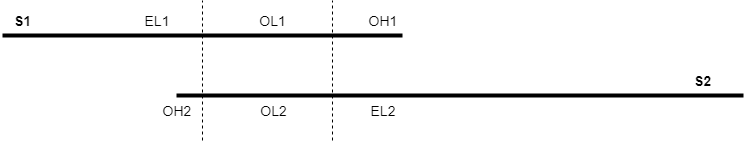
\includegraphics[width=\textwidth]{img/overlap.png}
\caption{Primjer preklapanja između S1 i S2}
\label{fig:overlap}
\end{figure}

Za preostale sekvence se računaju mjere preklapanja i produživanja. Na slici \ref{fig:overlap} je prikazano preklapanje između sekvenca $S_1$ i $S_2$ gdje se sekvenca $S_2$ nalazi nakon sekvence $S_1$. U sredini između isprekidanih linija je regija preklapanja čija je duljina $OL_1$ i $OL_2$, ovisno koju sekvencu gledamo, a izvana su $OH$ \engl{overhang length} i $EL$ \engl{extension length}. Koristeći navedene duljine, računa se mjera preklapanja $OS$ i mjere produživanja $ES_1$ i $ES_2$ prema izrazima \ref{eq:os} - \ref{eq:es2}. Pri tome je potrebno voditi računa preklapaju li se sekvence na istim lancima ili na suprotnim. Primjerice da se $S_1$ i $S_2$ preklapaju na suprotnim lancima, potrebno bi bilo zamijeniti vrijednosti $OH_2$ i $EL_2$.

\begin{equation}
OS = \frac{(OL_1 + OL_2) * SI}{2}
\label{eq:os}
\end{equation}
\begin{equation}
ES_1 = OS + \frac{EL_1}{2} - \frac{OH_1 + OH_2}{2}
\label{eq:es1}
\end{equation}
\begin{equation}
ES_2 = OS + \frac{EL_2}{2} - \frac{OH_1 + OH_2}{2}
\label{eq:es2}
\end{equation}

\section{Graf preklapanja}
Nakon što su sve mjere izračunate može se izgraditi graf preklapanja. Čvorovi u grafu predstavljaju contig-e i očitanja, a grane preklapanja, s time da grana može biti povezana na glavu ili rep čvora. Drugim riječima, svaki čvor ima svoje prefikse i sufikse. Sljedeći korak je traženje puteva između dva contig-a koji se obavlja pretraživanjem u dubinu \engl{DFS} uz nekoliko pravila. Postupak kreće iz svakog contig-a i zaustavlja se kada dođe do očitanja koje je povezano s drugim contig-om ili je trenutni put veći od maksimalne dopuštene duljine. Dodatno ograničenje je da se jedno očitanje ne može više puta pojaviti u istom putu.

Za izgradnju puteva koriste se tri pristupa. Prvi pristup iz početnog contiga izabere sve sufikse, ali za svako sljedeće produživanje bira ono koje ima najveću mjeru preklapanja $OS$. Ukoliko se dođe do čvora koji nema produživanja, vraća se jedan korak nazad i bira sljedeće najbolje produživanje. Drugi pristup radi isto kao prvi jedino koristi mjeru produživanja $ES$. Konačno, treći pristup nasumično bira produživanja proporcionalno mjeri produživanja $ES$, s time da je potrebno odrediti koliko puta će se iz svakog contig-a pokušati pronaći put ovom metodom. Po završteku postupka pronalaženja puteva između contig-a potrebno je samo odbaciti duplikate i moguće je prijeći na sljedeći korak algoritma.

\section{Stevo}

\section{Mihaela}
\chapter{Rezultati}
\chapter{Zaklju\v{c}ak}


Implementacija pomalo obskurnog i loše napisanog algoritma nam je donijela brojne probleme i natjerala nas da se fokusiramo više na maštu i vlastitu reimplementaciju. Napravili smo dosta promjena u radu. Neke iz neshvaćanja, a neke jer su nam naše implementacije bolje radile. Poigravali smo se s različitim načinima filtriranja te razrješavanjem konsenzusa grupa. Sami rezultati nisu bajni, ali postoji još puno mjesta za napredak. Nismo se pozabavili stvarima poput drugačijih mjera za razješavanje konsenzusa grupa te nismo pretraživali u suprotnom smjeru od contige jer u tom slučaju bismo morali započeti pretragu ne samo od glave do repa već i od repa do glave svake contige što bi dodatno zakompliciralo implementaciju te produljilo sam rad algoritma. Isto tako samo promatramo SI mjeru prilikom razrješavanja puteva i nije nam se isplatilo komplicirati implementaciju u slučaju da putevi imaju jednaku važnost.




\bibliography{literatura}
\bibliographystyle{fer}

\end{document}
